\documentclass[aspectratio=169]{beamer}

% Document class and style
\usepackage{balance}

% Encoding and font settings
\usepackage[utf8]{inputenc}
\usepackage[T1]{fontenc}

% Hyperlinks and URLs
\usepackage{bookmark}
\usepackage{hyperref}
\usepackage{url}

% Tables and arrays
\usepackage{booktabs}
\usepackage{tabularx}
\usepackage{tabularray}
\usepackage{array}
\usepackage{multirow}
\usepackage{makecell}

% Mathematical symbols and fonts
\usepackage{amsfonts}
\usepackage{amsmath}
\usepackage{nicefrac}

% Typography and text enhancements
\usepackage{microtype}
\usepackage{soul}
\usepackage{xcolor}
\usepackage{calc}
\usepackage{listofitems}
\usepackage{csquotes}
\usepackage{xspace}
% \usepackage{arev}
\usepackage{pifont}
\usepackage{enumitem}
\usepackage{ulem}
\usepackage{soul}

% Floats and positioning
\usepackage{float}
\usepackage{dblfloatfix}
\usepackage{cuted}

% Graphics and plots
\usepackage{graphicx}
\usepackage{pgfplots}
\usepackage{subcaption}
\usepackage{multicol}
\pgfplotsset{compat=1.18}

% TikZ libraries for advanced drawing
\usepackage{tikz}
\usetikzlibrary{decorations.pathreplacing}
\usetikzlibrary{arrows.meta}
\usetikzlibrary{matrix}
\usetikzlibrary{calc}
\usetikzlibrary{fit}
\usetikzlibrary{decorations.pathmorphing}
\usetikzlibrary{shapes}
\usetikzlibrary{positioning}
\usetikzlibrary{patterns}
\usetikzlibrary{backgrounds}
\usetikzlibrary{plotmarks}
\tikzset{>=latex}   % Set the default arrowhead style for TikZ drawings to 'latex'
\usepackage[outline]{contour}   % Load the 'contour' package with the 'outline' option
\contourlength{1.2pt}   % Set the thickness of the outline created by the 'contour' package

% Conditional statements and loops
\usepackage{comment}
\usepackage{nameref}
\usepackage{pgffor}
\usepackage{ifthen}
\usepackage{etoolbox}
\usepackage{iflang}

\usepgfplotslibrary{fillbetween}
\colorlet{myred}{red!60!black}
\colorlet{mygreen}{green!50!black}
\colorlet{myblue}{blue!80!black}

\lstset{
    basicstyle=\ttfamily\footnotesize,
    keywordstyle=\color{blue},
    commentstyle=\color{gray},
    stringstyle=\color{orange},
    numbers=left,
    numberstyle=\tiny,
    breaklines=true,
    frame=single,
}

\setbeamertemplate{navigation symbols}{}
\setbeamertemplate{page number in head/foot}[totalframenumber]
\setbeamertemplate{footline}{
  \leavevmode%
  \hbox{%
    \begin{beamercolorbox}[wd=\paperwidth,ht=2.5ex,dp=1ex,right]{page number in head/foot}%
      \usebeamerfont{page number in head/foot}%
      \usebeamertemplate*{page number in head/foot}%
      \hspace*{2ex}
    \end{beamercolorbox}%
  }%
}

\title{RLlib: Industry-Grade, Scalable Reinforcement Learning}
\author{
  Maxime Alaarabiou\\
}
\date{}

\begin{document}

\frame{\titlepage}

\begin{frame}{}
    \begin{figure}
    \centering
    \resizebox{\textwidth}{!}{
    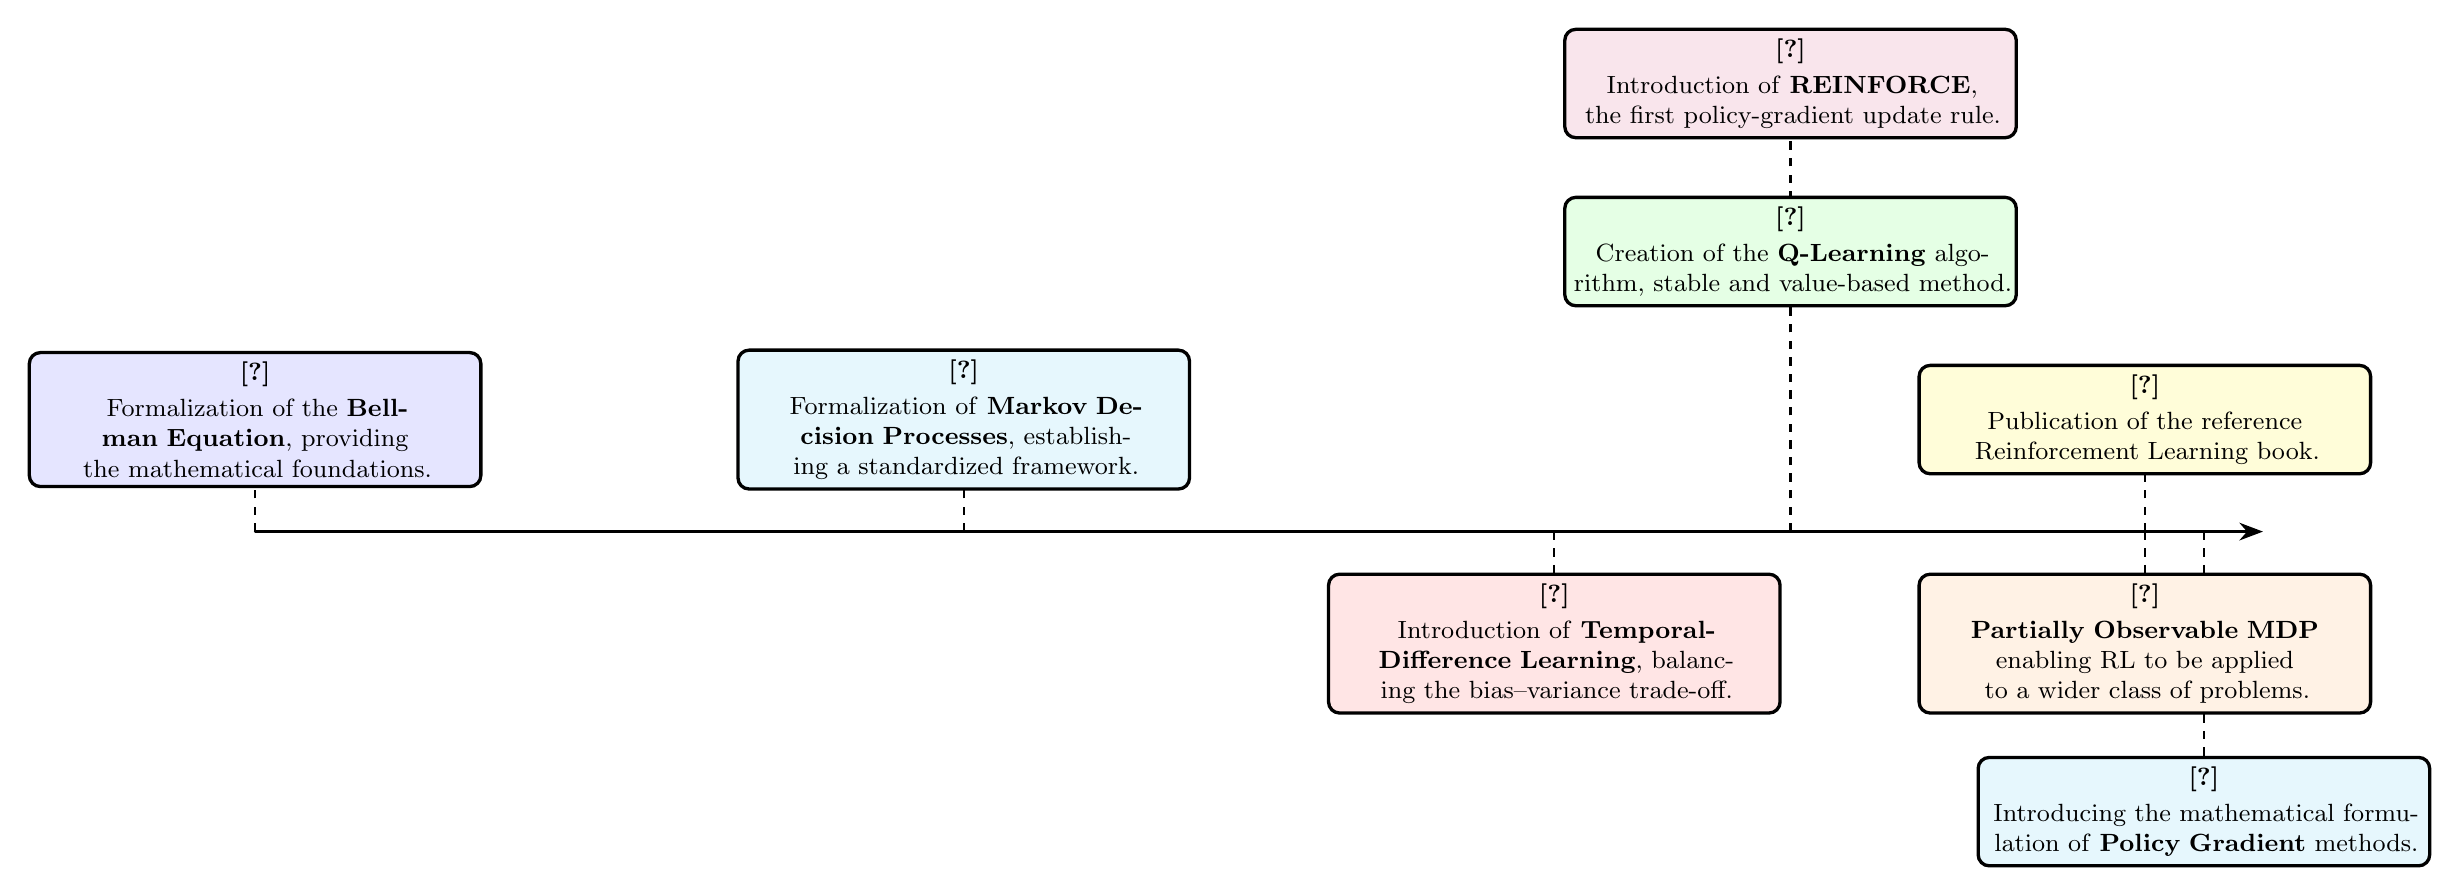
\begin{tikzpicture}[
        timeline/.style={draw, thick, -{Stealth[length=3mm]}, line cap=round},
        connect/.style={thick, dashed}
    ]

    %=== Timeline scale parameters ===%
    \def\yearmin{1966}
    \def\yearmax{2000}
    \def\scalefactor{0.75} % cm per year, to fit everything

    % Main timeline
    \draw[timeline] (0,0) -- ({(\yearmax-\yearmin)*\scalefactor},0);

    %=== Event Macro ===%
    \newcommand{\event}[8]{
        \pgfmathsetmacro{\x}{(#1-\yearmin)*\scalefactor}
        \pgfmathsetmacro{\y}{#6}

        \begin{scope}[on background layer]
            \draw[connect] (\x,0) -- ++(0,\y);
        \end{scope}

        \node[
            draw,
            rounded corners,
            very thick,
            fill=#8,
            minimum height=#5,
            text width=#4,
            align=center,
            font=#7
        ] at (\x, \y) {\textbf{\cite{#2}} \\[2pt] #3};
    }

    %=== EVENTS ===%

    \event{1966}{bellman1966dynamic}{
    Formalization of the \textbf{Bellman Equation}, providing the mathematical foundations.}{5.5cm}{1cm}{0.05cm}{\small}{blue!10};

    \event{1978}{puterman1978modified}{
        Formalization of \textbf{Markov Decision Processes}, establishing a standardized framework.}{5.5cm}{1cm}{0.05cm}{\small}{cyan!10};

    \event{1988}{sutton1988learning}{
        Introduction of \textbf{Temporal-Difference Learning}, balancing the bias--variance trade-off.}{5.5cm}{1cm}{-0.05cm}{\small}{red!10};

    \event{1992}{watkins1992q}{
        Creation of the \textbf{Q-Learning} algorithm, stable and value-based method.}{5.5cm}{1cm}{0.125cm}{\small}{green!10};

    \event{1992}{williams1992simple}{
        Introduction of \textbf{REINFORCE}, the first policy-gradient update rule.}{5.5cm}{1cm}{0.2cm}{\small}{purple!10};

    \event{1998}{kaelbling1998planning}{
        \textbf{Partially Observable MDP} enabling RL to be applied to a wider class of problems.}{5.5cm}{1cm}{-0.05cm}{\small}{orange!10};

    \event{1998}{sutton2018reinforcement}{
        Publication of the reference Reinforcement Learning book.}{5.5cm}{1cm}{0.05cm}{\small}{yellow!15};

    \event{1999}{sutton1999policy}{
        Introducing the mathematical formulation of \textbf{Policy Gradient} methods.}{5.5cm}{1cm}{-0.125cm}{\small}{cyan!10};


    \end{tikzpicture}
    }
\end{figure}

\end{frame}
\begin{frame}{}
    \begin{figure}
    \centering
    \resizebox{\textwidth}{!}{
    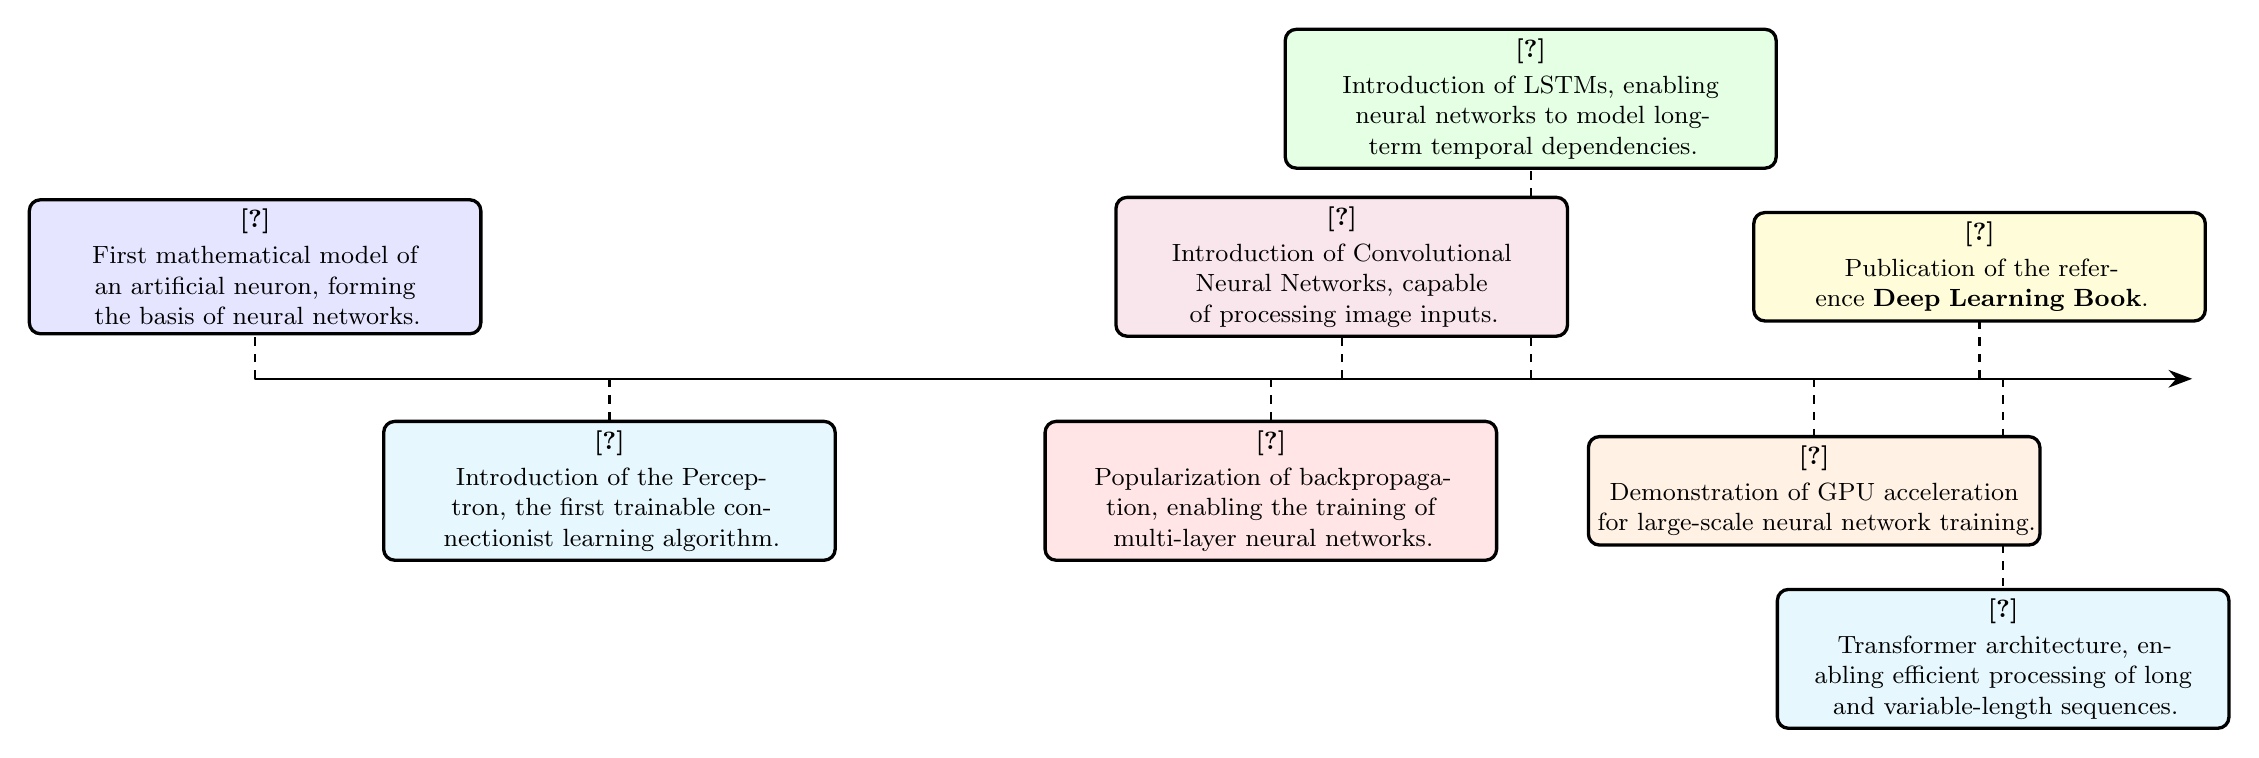
\begin{tikzpicture}[
        timeline/.style={draw, thick, -{Stealth[length=3mm]}, line cap=round},
        connect/.style={thick, dashed}
    ]

    %=== Timeline scale parameters ===%
    \def\yearmin{1943}
    \def\yearmax{2025}
    \def\scalefactor{0.3} % cm per year, to fit everything

    % Main timeline
    \draw[timeline] (0,0) -- ({(\yearmax-\yearmin)*\scalefactor},0);

    %=== Event Macro ===%
    \newcommand{\event}[8]{
        \pgfmathsetmacro{\x}{(#1-\yearmin)*\scalefactor}
        \pgfmathsetmacro{\y}{#6}

        \begin{scope}[on background layer]
            \draw[connect] (\x,0) -- ++(0,\y);
        \end{scope}

        \node[
            draw,
            rounded corners,
            very thick,
            fill=#8,
            minimum height=#5,
            text width=#4,
            align=center,
            font=#7
        ] at (\x, \y) {\textbf{\cite{#2}} \\[2pt] #3};
    }

    %=== EVENTS ===%
    \event{1943}{mcculloch1943logical}{
    First mathematical model of an artificial neuron, forming the basis of neural networks.}{5.5cm}{1cm}{0.05cm}{\small}{blue!10};

    \event{1958}{rosenblatt1958perceptron}{
    Introduction of the Perceptron, the first trainable connectionist learning algorithm.}{5.5cm}{1cm}{-0.05cm}{\small}{cyan!10};

    \event{1986}{rumelhart1986learning}{
    Popularization of backpropagation, enabling the training of multi-layer neural networks.}{5.5cm}{1cm}{-0.05cm}{\small}{red!10};

    \event{1989}{lecun1989backpropagation}{
    Introduction of Convolutional Neural Networks, capable of processing image inputs.}{5.5cm}{1cm}{0.05cm}{\small}{purple!10};

    \event{1997}{hochreiter1997long}{
    Introduction of LSTMs, enabling neural networks to model long-term temporal dependencies.}{6cm}{1cm}{0.125cm}{\small}{green!10};

    \event{2009}{raina2009large}{
    Demonstration of GPU acceleration for large-scale neural network training.}{5.5cm}{1cm}{-0.05cm}{\small}{orange!10};

    \event{2016}{Goodfellow-et-al-2016}{
    Publication of the reference \textbf{Deep Learning Book}.}{5.5cm}{1cm}{0.05cm}{\small}{yellow!15};

    \event{2017}{vaswani2017attention}{
    Transformer architecture, enabling efficient processing of long and variable-length sequences.}{5.5cm}{1cm}{-0.125cm}{\small}{cyan!10};
    \end{tikzpicture}
    }
\end{figure}

\end{frame}
\begin{frame}{}
    \begin{figure}
    \centering
    \resizebox{\textwidth}{!}{
    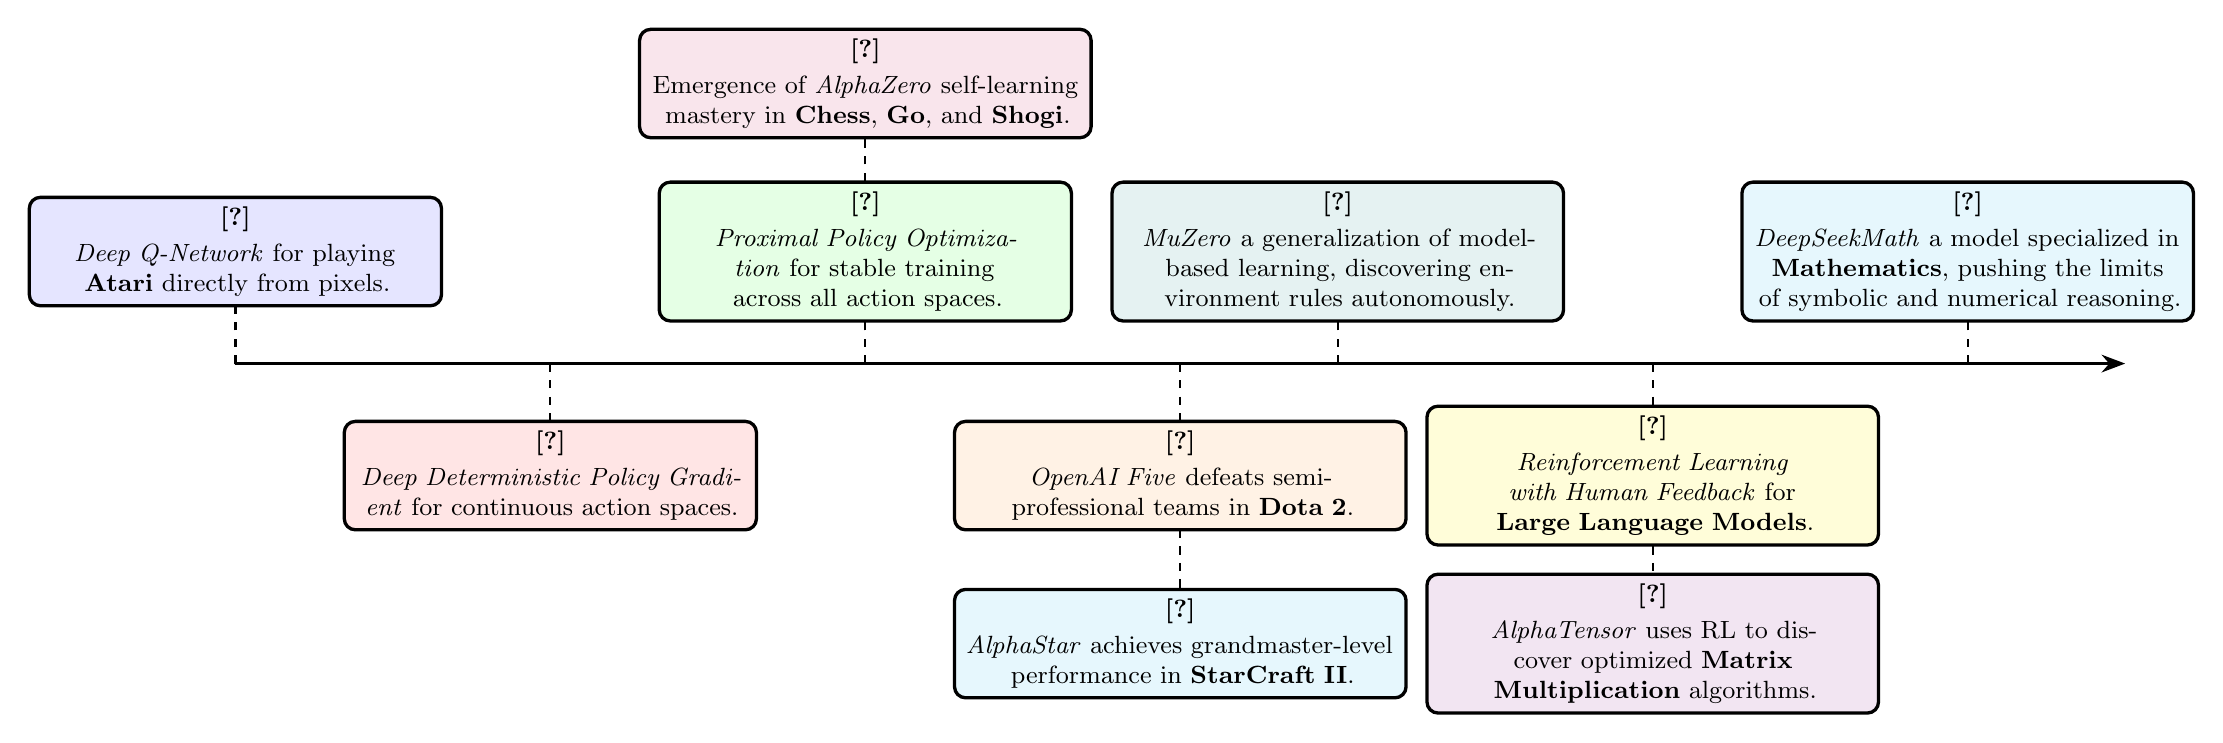
\begin{tikzpicture}[
        timeline/.style={draw, thick, -{Stealth[length=3mm]}, line cap=round},
        connect/.style={thick, dashed}
    ]

    %=== Timeline scale parameters ===%
    \def\yearmin{2013}
    \def\yearmax{2025}
    \def\scalefactor{2} % cm per year

    % Main line
    \draw[timeline] (0,0) -- ({(\yearmax-\yearmin)*\scalefactor},0);

    %=== Macro to place events ===%
    % #1 = year
    % #2 = citation (bib key)
    % #3 = text
    % #4 = bubble width (text width)
    % #5 = minimum height of the bubble
    % #6 = Y offset
    % #7 = text size (e.g., \small)
    % #8 = bubble color (e.g., blue!10, red!15, green!20)
    \newcommand{\event}[8]{
        % Event position
        \pgfmathsetmacro{\x}{(#1-\yearmin)*\scalefactor}
        \pgfmathsetmacro{\y}{#6}

        % Connection line behind bubbles
        \begin{scope}[on background layer]
            \draw[connect] (\x,0) -- ++(0,\y);
        \end{scope}

        % Bubble in the foreground
        \node[
            draw,
            rounded corners,
            very thick,
            fill=#8,
            minimum height=#5,
            text width=#4,
            align=center,
            font=#7
        ] (E#1) at (\x, \y) {\textbf{\cite{#2}} \\[2pt] #3};
    }

    %=== Events ===%
    \event{2013}{mnih2013playing}{
    \textit{Deep Q-Network} for playing \textbf{Atari} directly from pixels.}{5cm}{1cm}{0.05cm}{\small}{blue!10};

    \event{2015}{lillicrap2019continuouscontroldeepreinforcement}{
    \textit{Deep Deterministic Policy Gradient} for continuous action spaces.}{5cm}{1cm}{-0.05cm}{\small}{red!10};

    \event{2017}{schulman2017proximal}{
    \textit{Proximal Policy Optimization} for stable training across all action spaces.}{5cm}{1cm}{0.05cm}{\small}{green!10};

    \event{2017}{silver2017masteringchessshogiselfplay}{
    Emergence of \textit{AlphaZero} self-learning mastery in \textbf{Chess}, \textbf{Go}, and \textbf{Shogi}.}{5.5cm}{1cm}{0.125cm}{\small}{purple!10};

    \event{2019}{berner2019dota}{
    \textit{OpenAI Five} defeats semi-professional teams in \textbf{Dota 2}.}{5.5cm}{1cm}{-0.05cm}{\small}{orange!10};

    \event{2019}{vinyals2019grandmaster}{
    \textit{AlphaStar} achieves grandmaster-level performance in \textbf{StarCraft II}.}{5.5cm}{1cm}{-0.125cm}{\small}{cyan!10};

    \event{2020}{Schrittwieser_2020}{
    \textit{MuZero} a generalization of model-based learning, discovering environment rules autonomously.}{5.5cm}{1cm}{0.05cm}{\small}{teal!10};

    \event{2022}{ouyang2022training}{
    \textit{Reinforcement Learning with Human Feedback} for \textbf{Large Language Models}.}{5.5cm}{1cm}{-0.05cm}{\small}{yellow!15};

    \event{2022}{fawzi2022discovering}{
    \textit{AlphaTensor} uses RL to discover optimized \textbf{Matrix Multiplication} algorithms.}{5.5cm}{1cm}{-0.125cm}{\small}{violet!10};

    \event{2024}{shao2024deepseekmathpushinglimitsmathematical}{
    \textit{DeepSeekMath} a model specialized in \textbf{Mathematics}, pushing the limits of symbolic and numerical reasoning.}{5.5cm}{1cm}{0.05cm}{\small}{cyan!10};

    \end{tikzpicture}
    }
\end{figure}

\end{frame}

\begin{frame}{}
    \begin{figure}
    \centering
    \resizebox{\textwidth}{!}{
    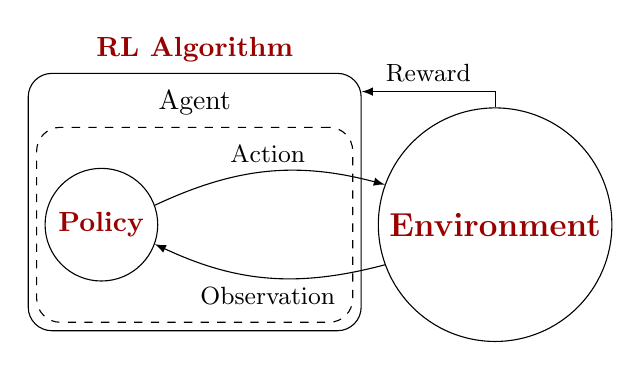
\begin{tikzpicture}
        \sethlcolor{myred}
        % Nodes
        \node[draw, circle, align=center] (policy) at (-5, 0) {\textcolor{myred}{\textbf{Policy}}};
        \node[draw, circle, align=center] (environment) at (0, 0) {\large \textcolor{myred}{\textbf{Environment}}};
    
        % Arrows with labels
        \draw[->, bend left=20] (policy) to node[above, font=\small, align=center] (action) {Action} (environment);
        \draw[->, bend left=20] (environment) to node[below, font=\small, align=center] (observation) {Observation} (policy);

        % Agent
        \node[draw, rectangle, fit=(policy)(action)(observation), inner sep=0.1cm, dashed, rounded corners=0.3cm] (agent_box) {};
        \node[] (agent_label) at ($(agent_box.north) + (0, 0.3cm)$) {Agent};

        % RL Algorithm
        \node[draw, rectangle, fit=(agent_box)(agent_label), inner sep=0.1cm, rounded corners=0.3cm] (rl_algorithm_box) {};
        \node[] (rl_algorithm_label) at ($(rl_algorithm_box.north) + (0, 0.3cm)$) {\textcolor{myred}{\textbf{RL Algorithm}}};
        
        % Reward
        \coordinate (top_environment) at ($(environment.north) + (0, 0.2cm)$);
        \coordinate (point_rl_algorithm_box) at (rl_algorithm_box.east |- top_environment);
        \draw[->] (environment.north) -- (top_environment) -- node[above, font=\small] {Reward} (point_rl_algorithm_box);
    \end{tikzpicture}
    }
\end{figure}
\end{frame}
\begin{frame}[fragile]{}
\centering
\textbf{Gymnasium:}

{\scriptsize
\begin{lstlisting}[language=Python]
import gymnasium as gym

env = gym.make("ALE/SpaceInvaders-v5", render_mode="rgb_array")
obs, info = env.reset()
action = env.action_space.sample()
obs, reward, terminated, truncated, info = env.step(action)
\end{lstlisting}
}

\vspace{0.4cm}
\textbf{PettingZoo:}

{\scriptsize
\begin{lstlisting}[language=Python]
from pettingzoo.atari import space_invaders_v2

env = space_invaders_v2.env(render_mode="rgb_array")
env.reset()
for agent in env.agent_iter():
    obs, reward, term, trunc, info = env.last()
    action = env.action_space(agent).sample() if not term else None
    env.step(action)
\end{lstlisting}
}

\end{frame}

\begin{frame}[fragile]
\vfill
\centering
\footnotesize
\resizebox{0.5\textwidth}{!}{
\begin{tabular}{>{\ttfamily}l l}
\toprule
\multicolumn{2}{c}{\textbf{Environment Configuration}} \\
\midrule
game\_name & 'SpaceInvaders-v5' \\
repeat\_action\_probability & 0.05 \\
frameskip & 5 \\
resize\_observation\_shape & (64, 64) \\
convert\_to\_grayscale & True \\
reward\_scale\_factor & 0.05 \\
frame\_stack\_len & 4 \\
normalize\_observation & True \\
observation\_numpy\_type & np.float16 \\
\midrule
\multicolumn{2}{c}{\textbf{Policy Architecture Configuration}} \\
\midrule
architecture & CnnPPO \\
configuration\_cnn & [(16,4,2),(32,4,2),(64,4,2),(128,4,2)] \\
configuration\_hidden\_layers & [512,256,128] \\
activation\_function\_class & LeakyReLU \\
use\_layer\_normalization\_cnn & True \\
use\_share\_cnn & True \\
\midrule
\multicolumn{2}{c}{\textbf{Reinforcement Learning Configuration}} \\
\midrule
algorithm\_name & 'PPO' \\
rollout\_fragment\_length & 2048 \\
train\_batch\_size & 2048 * 8 \\
minibatch\_size & 2048 \\
lambda\_gae & 0.95 \\
kullback\_leibler\_coefficient & 0.5 \\
clip\_policy\_parameter & 0.1 \\
clip\_value\_function\_parameter & 10 \\
entropy\_coefficient & 0.01 \\
number\_epochs & 10 \\
learning\_rate & 0.00015 \\
gradient\_clip & 100.0 \\
gradient\_clip\_by & 'global\_norm' \\
\bottomrule
\end{tabular}
}
\vfill
\end{frame}

\begin{frame}[plain]
\centering
\vspace{0.2cm}
{\LARGE \textcolor{myblue}{\textbf{Why choose RLlib?}}}\\[0.5cm]

\begin{itemize}
    \centering
    \item \textbf{Open-source} and actively maintained
    \item \textbf{Scalable} from laptop to large compute clusters
    \item Supports many modern algorithms: \textbf{DQN, DDPG, PPO, Dreamer, …}
    \item \textbf{Customizable Policy Architecture}: Dense, CNN, LSTM, Attention
    \item Compatible with both \textbf{PyTorch} and \textbf{TensorFlow}
    \item \textbf{Automatic Plotting} of training curves
    \item \textbf{Automatic Checkpointing and Restart} of training
    \item \textbf{Multi-agent} and \textbf{Hierarchical} RL
    \item \textbf{Advanced Callback System} for monitoring and customization
    \item Modules for \textbf{Exploration}, \textbf{Curriculum Learning}, and \textbf{Custom RL Algorithms}
\end{itemize}

\end{frame}


\begin{frame}[fragile]{}
\centering

{\scriptsize
\begin{lstlisting}[language=Python]
from ray.rllib.algorithms.ppo import PPOConfig
from pprint import pprint

# Configure the algorithm.
config = (
    PPOConfig()
    .environment("ALE/SpaceInvaders-v5")
)

# Build the algorithm.
algo = config.build_algo()
# Train it for 5 iterations ...
for _ in range(5):
    pprint(algo.train())
# ... and evaluate it.

pprint(algo.evaluate())
# Release the algo's resources.
algo.stop()
\end{lstlisting}
}

\end{frame}


\begin{frame}
    \begin{center}
        \vfill
        {\bfseries\Huge \textcolor{myblue}{Thank you for your attention}}

        \vspace{0.2cm}

        \color{gray}
        \Large Questions, Comments, Ideas?
        \vfill
    \end{center}
\end{frame}


\bibliographystyle{apalike}
\bibliography{
  references/classic_reinforcement_learning,
  references/deep_learning,
  references/deep_reinforcement_learning,
}

\end{document}
